\documentclass[tikz, dvipsnames]{standalone}


\usepackage{amsmath}

\begin{document}
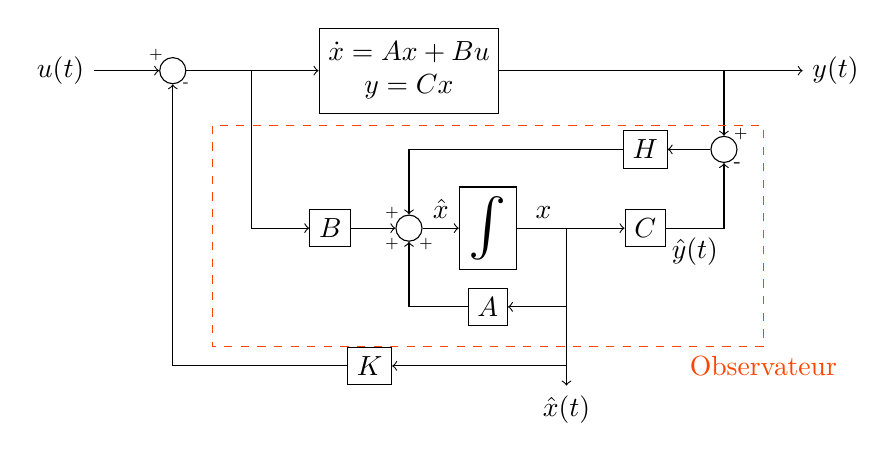
\begin{tikzpicture}
\coordinate (A) at (-1,0);
\coordinate (A2) at (0,0);
\coordinate (B) at (1,0);
\coordinate (C) at (3,0);
\coordinate (D) at (5,0);
\coordinate (E) at (2,-2);
\coordinate (F) at (3,-2);
\coordinate (G) at (4,-2);
\coordinate (H) at (4,-3);
\coordinate (I) at (5,-2);
\coordinate (J2) at (5,-3.75);
\coordinate (J3) at (2.5,-3.75);
\coordinate (J) at (5,-4);
\coordinate (K) at (6,-2);
\coordinate (L) at (7,-1);
\coordinate (M) at (6,-1);
\coordinate (N) at (8,0);


\node[anchor=east] at (A) {$u(t)$};

\node[rectangle,draw] (c) at (C) {$\begin{matrix}\dot{x}=Ax+Bu\\y=Cx\end{matrix}$};

\node[rectangle,draw] (e) at (E) {$B$};
\node[circle,draw] (f) at (F) {};
\node[circle,draw] (a2) at (A2) {};
\node[rectangle,draw] (g) at (G) {\huge $\int$};
\node[rectangle,draw] (h) at (H) {$A$};
\node[anchor=north] at (J) {$\hat{x}(t)$};
\node[rectangle,draw] (k) at (K) {$C$};
\node[circle,draw] (l) at (L) {};
\node[rectangle,draw] (m) at (M) {$H$};
\node[anchor=west] at (N) {$y(t)$};
\node[rectangle,draw] (j3) at (J3) {$K$};

\draw[->] (A) -- (a2) node[anchor=south east] {\tiny +};
\draw[->] (a2) -- (c);
\draw[->] (B) |- (e);
\draw[->] (e) -- (f) node[anchor=north east] {\tiny +};
\draw[->] (f) -- (g) node[midway,anchor=south] {$\hat{x}$};
\draw[->] (h) -| (f) node[anchor=north west] {\tiny +};
\draw[->] (I) |- (h);
\draw[->] (I) -- (J);
\draw[->] (g) -- (k) node[pos=0.25,anchor=south] {$x$};
\draw[->] (k) -| (l) node[anchor=north west] {\scriptsize -} node[pos=0.25,anchor=north] {$\hat{y}(t)$};
\draw[->] (l) -- (m);
\draw[->] (m) -| (f) node[anchor=south east] {\tiny +};
\draw[->] (c) -- (N);
\draw[->] (c) -| (l) node[anchor=south west] {\tiny +};

\draw[->] (J2) -- (j3);
\draw[->] (j3) -| (a2) node[anchor=north west] {\tiny -};

\draw[OrangeRed,dashed] (0.5,-0.7) rectangle (7.5,-3.5) node[below] {Observateur};






\end{tikzpicture}
\end{document}